\subsection{Introducción al CFD}\label{header-n0}

El principal cometido de las ciencias naturales es describir la realidad
con la mayor precisión posible para entender mejor el fenómeno natural.
En ingeniería el propósito de las investigaciones se centran en
desarrollar nuevos productos y optimizar los existentes.

En el pasado existían dos aproximaciones científicas: la experimental y
la teórica o el análisis dimensional. Con la llegada de los ordenadores
fue posible una nueva aproximación: las simulaciones numéricas.

Las ecuaciones matemáticas que describen los fenómenos físicos de la
naturaleza con una precisión razonable, suelen ser tan complejas que no
es posible obtener una solución analítica. {[}Fuente: M. de Mier,
2004{]}

\subsubsection{Definición de CFD}\label{header-n8}

Acrónimo, adoptado del inglés \emph{Computational Fluid Dynamics}, que
hace referencia a la rama de la Mecánica de Fluidos y más concretamente
a la \textbf{Dinámica de Fluidos Computacional}. Consiste en el empleo
de métodos numéricos y algoritmos para estudiar y analizar problemas que
involucran fluidos en movimiento, mediante la solución de las ecuaciones
de Navier-Stokes, transferencia de calor, entre otras, por ordenador.
Existen diferentes métodos numéricos y algoritmos que resuelven de
distinta forma las ecuaciones fundamentales.
\href{http://docplayer.es/720690-Simulacion-de-fluidos-utilizando-computadores-una-moderna-herramienta-para-el-estudio-y-analisis-de-fluidos.html}{Fuente:
Una moderna herramienta para el estudio y analisis de fluidos}

En general, el CFD comprende un amplio abanico de disciplinas
científicas, entre las que destacan las matemáticas, la programación,
las ciencias físicas y la ingeniería, que deben aunarse para dar lugar
al desarrollo de un código que sea capaz de resolver las ecuaciones de
flujo de manera satisfactoria.

Por tanto, el objetivo final de un programa numérico (software) es
proporcionar el cálculo detallado del movimiento de los fluidos,
mediante un ordenador capaz de ejecutar gran cantidad de cálculos por
unidad de tiempo y resolver, así, las ecuaciones matemáticas que
expresan las leyes por las que se rigen los fluidos.

\subsubsection{Historia del CFD}\label{header-n15}

Hace ya casi dos siglos desde que las ecuaciones de gobierno de la
Mecánica de Fluidos quedaron definitivamente formuladas por Navier y
Stokes cuando introdujeron los términos de transporte viscoso a las
ecuaciones de Euler, dando lugar a las ecuaciones de Navier-Stokes.
Estas ecuaciones incluyen las leyes de conservación para la masa, la
cantidad de movimiento y la energía de un flujo. De ahí se obtiene un
sistema acoplado de ecuaciones del que no es posible hallar una solución
analítica única.

En el siglo XX, asentadas las bases teóricas de la Mecánica de Fluidos,
se comenzaron las investigaciones sobre la capa límite y la turbulencia
(esta última sigue siendo uno de los mayores retos). Von Kárman estudió
el desprendimiento de vórtices en las estelas de cuerpos en flujo
externo. Kolmogorov definió el concepto del espectro universal de
energía de la turbulencia y de la cascada de energía. Lewis Fry
Richardson, precursor de la utilización de las técnicas CFD, fue el
primero en utilizar un motelo matemático para la metereología entre
1910-1920. Profetizando el cálculo en paralelo, Brian Spalding en 1970
define uan fórmula empírica en términos de velocidad y presión,
introduciendo por primera vez el método de acoplamiento SIMPLE. Como más
tarde se verá, los métodos implícitos tienen una clara ventaja frente a
los explicitos, ya que no presentan restricciones en la discretización
temporal, garantizando siempre la estabilidad numérica. Más tarde se
desarrollaron modificaciones y mejoras del modelo de acoplamiento (PISO,
PIMPLE, ...).

Sushas V. Patankar publicó "Numerical Heat Transfer and Fluid Flow",
probablemente el primer gran libro que trata en profundidad las
metodologías CFD y que ha servido de inspiración para la creación de
infinidad de códigos numéricos. Patankar y el Imperial Collage, sientan
las bases definitivas del método de volúmenes finitos. El auge de estas
técnicas, junto con los avances de la tecnología, llevó a la industria
aeronáutica y aeroespacial a lanzarse por el empleo del CFD en fases de
diseño y verificación de modelos.

A partir del, 2003 se produce una importante concentración de paquetes
iniciada por ANSYS (lider mundial en desarrollo de herramientas de
análisis en el campo de la ingeniería asistida por ordenador (CAE)
haciéndose con la compra del código numérico CFX y tres años después de
FLUENT) y CD-Adapco (heredera del código STAR-CD y participada por la
empresa de CAD Dassault Systems (fabricante de CATIA) han dado lugar a
un progresivo incremento en los precios de las licencias. Sin embargo,
esta técnica puede verse contrarrestada con la aparición de nuevos
códigos numéricos de distribución libres, como Linux. El pionero en la
creación de códigos libres de CFD es OpenFOAM.

Hoy en día, se están reemlazando caros experimentos por simulaciones por
ordenador. Así mismo, su utilización se ha extendido a todo tipo de
procesos industriales, gracias a la universalización de los códigos y a
la progresiva mejora de los algoritmos que implementan. Siendo la
industria aeroespacial pionera en el empleo de estas herramientas, le
siguieron: la industria automovilística, la aeronáutica, naval,
fabricación de motores, generación eléctrica, química, electrónica,
nuclear, biomédica, entre otras.

\subsubsection{Ventajas e Inconvenientes}\label{header-n26}

El uso de las técnicas CFD ofrecen numerosas ventajas, entre ellas se
destaca la posibilidad casi ilimitada de obtener valiosa información,
como por ejemplo, en situaciones en las que la experimentación no es
segura, no es abordable por una empresa (líneas de fabricación que no
pueden ser alteradas) o sencillamente no es viable (condiciones de
ingravidez, reentradas aerospaciales).

Sin embargo, el \emph{hardware} y \emph{software} requerido para
ejecutar estas técnicas no está al alcance de todos, tanto por los
conocimientos requeridos (para dominar el programa y la gestión de
resultados), como por el equipo y precio de las licencias, cuando se
usan progamas comerciales.

A continuación, se listan las ventajas e inconvenientes más relevantes
del uso del CFD:

\begin{itemize}
\item
  Ventajas:

  \begin{itemize}
  \item
    Reducción sustancial de tiempos y costes en fases de diseño.
  \item
    Posibilidad de analizar sistemas o condiciones muy difíciles de
    reproducir experimentalmente.

    \begin{itemize}
    \item
      Velocidades hipersónicas, temperaturas extremas, movimientos
      relativos, etc.
    \end{itemize}
  \item
    Capacidad de estudiar sistemas bajo condiciones peligrosas.

    \begin{itemize}
    \item
      Accidentes, situaciones límite de equipos, etc.
    \end{itemize}
  \item
    Nivel de detalle prácticamente ilimitado.

    \begin{itemize}
    \item
      Facilidad para estudios paramétricos.
    \item
      Gran cantidad de información, sin costes añadidos por aumento de
      puntos de medición.
    \end{itemize}
  \item
    Visibilización de modelos con diseño asistido por ordenador.

    \begin{itemize}
    \item
      Un valor añadido al producto.
    \end{itemize}
  \end{itemize}
\item
  Inconvenientes:

  \begin{itemize}
  \item
    Las técnicas CFD no son baratas.

    \begin{itemize}
    \item
      Máquinas con gran capacidad de cálculo.
    \item
      Programas comerciales no asequibles para la gran mayoría.
    \end{itemize}
  \item
    Se necesita personal cualificado.

    \begin{itemize}
    \item
      Ejecutar el programa y definir los modelos.
    \item
      Analizar soluciones.
    \end{itemize}
  \item
    No siempre es posible obtener resultados lo suficientemente
    precisos.

    \begin{itemize}
    \item
      Necesidad de simplificar el fenómeno.
    \end{itemize}
  \item
    Limitación de los modelos existentes para la turbulencia, la
    combustión, flujos multifásicos, etc.
  \item
    Tendencia a dar por buenos los resultados sin la suficiente
    contrastación.
  \end{itemize}
\end{itemize}

\subsection{Ideas Fundamentales}\label{header-n109}

\subsubsection{Fluidos y Flujos}\label{header-n110}

Los fluidos son sustancias que no son capaces de resistir fuerzas
externas, hasta las fuerzas más pequeñas causan deformaciones en las
partículas del fluido. Aunque existan diferencias significantes entre
líquidos y gases, ambos obedecen a las mismas leyes de movimiento. Los
flujos son causados por diferencias de presión, gravedad, esfuerzo
cortante, rotación y tensiones superficiales. Las propiedades más
importantes de los fluidos son la densidad y viscosidad.

Un flujo es \textbf{incompresible} si la densidad del fluido (masa por
unidad de volumen) se puede asumir constante. Esto también se aplica a
los gases, si el número de Mach:

\[Ma=\frac{v}{c}=\frac {\text{velocidad de flujo}}{\text{velocidad del sonido}} < 0,3\]

es decir, los flujos de gases a altas velocidades. La incompresibilidad
no es una propiedad del fluido, pero sí del flujo.

La \textbf{viscosidad} de un fluido es la medida de su resistencia a la
deformación por cortadura. Se debe a la interacción entre las moléculas
del fluido, a medida que la temperatura aumenta, la viscosidad de los
líquidos disminuye, mientras que la de los gases aumenta.

En el flujo alejado de la superficie sólida, el efecto de la viscosidad
es, normalmente, menor. Un flujo no viscoso (Euler) no puede adherirse a
las paredes y se considera el deslizamiento en los limites de pared.

El \textbf{número de Reynolds} es un parámeto adimensional que expresa
la relación entre las fuerzas de inercia y las fuerzas de fricción en el
flujo:

\[Re= \frac{\rho u L}{\mu}\]

donde, \emph{u} es la velocidad característica del flujo, \emph{L} es la
longitud característica y \(\mu\) es la viscosidad dinámica.

Cuando la velocidad del flujo es muy baja, el fluido es muy viscoso o
las dimensiones de la geometría son muy pequeñas (esto es, cuando el
número de Reynods es pequeño), la convectividad (término de inercia) en
las ecuaciones de Navier-Stokes juega un papel menor y se puede
despreciar. En estos casos, el flujo se denomina progresivo,
\emph{creeping (Stokes) flow}.

A medida que la velocidad aumenta, y por tanto el número de Re, la
inercia se vuelve más importante, pero si cada partícula del fluido
sigue una trayectoria suabe, el flujo es \textbf{laminar}. Si los
efectos de la viscosidad dominan, las perturbaciones pueden ser
atenuadas. Aún así, si se sigue aumentando la velocidad se pruducirá un
flujo inestable con trayectorias variables, denominado flujo
\textbf{turbulento}. Los flujos turbulentos son transitorios,
irregulares, no lineales y caracterizados por las formaciones de
vórtices. A altas velocidades, el número de Reynolds es muy alto y los
efectos de la viscosidad y la turbulencia se hacen relevantes en las
regiones cercanas a las paredes, en capa límite (\emph{boundary layer}).
Para resolver esta capa, se necesita un refinado de la malla.

\begin{figure}
\centering
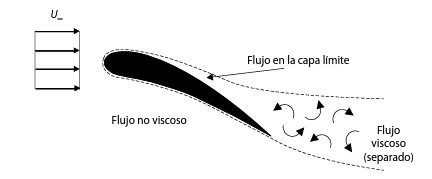
\includegraphics{31-flujoPerfil.jpg}
\caption{Zonas de flujo externo sobre un perfil aerodinámico}
\label{fig:flujoPerfil}
\end{figure}

Muchos flujos de interés práctico son difíciles de describir con
exactitud matemáticamente. Estos flujos incluyen turbulencia,
combustión, o multifásicos. A menudo, la solución exacta es imposible,
normalmente se usan modelos semi-empíricos para representar estos
fenómenos.

La \textbf{descripción lagrangiana} sigue el movimiento de una partícula
a través del espacio. La posición descrita por una partícula del fluido
en el tiempo es función de la posición inicial y el tiempo transcurrido.

La \textbf{descripción euleriana} se centra en un punto fijo en el
espacio y observa el paso de las partículas fluidas. La velocidad se
expresa como función del tiempo y la posición fija de referencia.

\subsubsection{3.2.2 Discretización espacial}\label{header-n143}

A diferencia de los problemas estáticos, donde sólo se requiere conocer
la densidad del fluido y la posición de la superficie libre, en la
mayoría de los problemas con flujos es necesario analizar un estado
arbitrario de movimiento del fluido definido por la geometría, las
condiciones de contorno y las leyes de la mecánica. Las tres técnicas
básicas del análisis de los problemas de flujos arbitrarios son:

\begin{enumerate}
\def\labelenumi{\arabic{enumi}.}
\item
  Volumen de control, o análisis integral a gran escala.
\item
  Diferencial, o análisis a pequeña escala.
\item
  Experimental, o análisis dimensional.
\end{enumerate}

La mayoría de los programas para el CFD, emplean la estrategia de
reemplazar un problema definido sobre un \textbf{dominio continuo}
(hipótesis del continuo en Mecánica de Fluidos clásica) por un
\textbf{dominio discreto} definido a partir de una malla. De esta
manera, cada variable del flujo (presión, velocidad, temperatura) pasa
de estar definida en todos los puntos del espacio, a los puntos (nodos)
de la malla. A este proceso se le denoina \textbf{discretización
espacial}.

Asímismo, las variables de interés se resuelven en los puntos que
definen la malla y los valores en otras posiciones se determinan
mediante interpolación.

Tanto las ecuaciones de gobierno en derivadas parciales como las
condiciones de contorno, están definidas matemáticamente mediante
variables continuas. Es posible aproximar estas complejas ecuaciones no
lineales por una serie de ecuaciones algebraicas que relacionan las
variables discretizadas (por cada celda). El sistema de ecuaciones
resultante es un gran conjunto de ecuaciones algebraicas acopladas en
variables discretas. Manipular y resolver este sistema (lo cual implica
un problema de inversión matricial) requiere un gran número de cálculos
repetitivos, que finalmente serán resueltos iterativamente por
ordenador.

La discretización, divide la solución del dominio en un número finito de
subdominios y según cómo estén organizados darán lugar a los siguientes
tipos de mallas:

\begin{itemize}
\item
  \textbf{Malla estructurada}: Definida así cuando cada nodo tiene el
  mismo número de elementos a su alrededor. Esto hace que la matriz
  algebraica del sistema de ecuaciones tenga una estructura regular,
  dando lugar a mayor precisión, tiempo de cálculo y consumo de memoria.
  No obstante, a menudo resulta difícil controlar la distribución de los
  nodos. Dentro de este grupo están:

  \begin{itemize}
  \item
    Mallas cartesianas uniformes y no uniformes: mallas ortogonales,
    para el caso de las no uniformes la división no es regular en todas
    las direcciones.
  \item
    Mallas \emph{body-fitted}: se hace curvilínea para asemejarla a la
    forma geométrica. Normalmente se emplean métodos sofisticados para
    mantener condiciones de continuidad y suavidad en el tamaño de las
    celdas. Las configuraciones más habituales son el mallado en H
    (\emph{H-mesh}), en C (C-\emph{mesh}), en O (\emph{O-mesh}) y en I
    (I-\emph{mesh}).
  \item
    Mallas multibloque: Consisten en una combinación de mallas
    estructuradas, que aplican diversas topologías en diferentes zonas
    del dominio. En este caso se pueden encontrar, mallados C-H, H-O-H,
    en forma de mariposa, esntre otras.
  \end{itemize}
\item
  \textbf{Malla no estructurada}: Se ha convertido en el estándar para
  uso industrial debido a la imposibilidad de generar mallas
  estructuradas de forma completamente automática sobre geometrías
  arbitrarias. Existen diversos algoritmos de generación de mallados,
  que cubren cualquier dominio tridimensional sin necesidad de conocer a
  priori las topologías constitutivas del mismo. Asímismo, se permite la
  adaptación local de la malla, mediante refinamientos o reducción del
  tamaño de celdas por algún critério basado en el gradiente del flujo o
  en estimación de errores.

  Puesto que cualquier geometría poligonal puede reducirse
  progresivamente a un conjunto de elementos triangulares y
  cuadriláteros, esta es la unidad básica de generación de celdas. Se
  consideran las siguientes tipologías:

  \begin{itemize}
  \item
    Mallas triangulares (2-D) o tetraédricas (3-D): Presentan una
    flexibilidad extrema para adaptarse al modelo.
  \item
    Mallas híbridas: Cuando se necesita analizar los fenómenos
    relacionados con la capa límite, el mallado no estructurado resulta
    deficiente, una solución es convinar el mallado estructurado en
    aquellas zonas para conectarlo, después, con el resto del dominio.
  \item
    Mallas cuadriláteras (2-D) o hexaédricas (3-D): Generalmente, estas
    formas resultan más eficientes que las triangulares, necesitando
    menores recursos de memoria.
  \end{itemize}
\end{itemize}

\begin{figure}
\centering
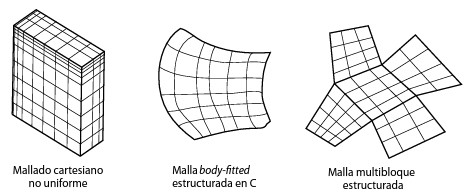
\includegraphics{32-mallaStruct.jpg}
\caption{Ejemplos de mallas estructuradas}
\label{fig:mallaStruct}
\end{figure}

\begin{figure}
\centering
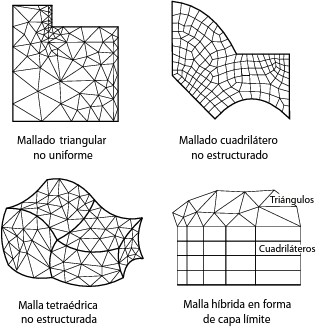
\includegraphics{32-mallaNOstruct.jpg}
\caption{Ejemplos de mallas no estructuradas}
\label{fig:mallaNOstruct}
\end{figure}

Cuando las soluciones numéricas que se obtienen en diferentes mallados
coinciden dentro de un nivel de tolerancia prefijado por el usuario, se
dice que dichas soluciones son \textbf{independientes de la malla}.

Tras la generación del mallado, el método de volúmenes finitos asocia un
volumen finito o local, también denominado \textbf{volumen de control},
a cada punto de la malla, y a continuación aplica las leyes integales de
conservación a cada volumen local.

La definición de los volúmenes de control, puede hacerse centrada en las
celdas o bien centrada en los vértices, aunque es práctica habitual
hacerlo en los centroides. No obstante, si las componentes de la
velocidad y las presiones se almacenan en las mismas posiciones, podrían
darse circunstancias irreales. Para evitarlo, se utiliza un
\textbf{mallado decalado (\emph{staggered grid})}, de forma que:

\begin{itemize}
\item
  Las variables \textbf{escalares}, como la presión, la temperatura o la
  fracción másica, se evalúan en los centros de las celdas
  (\emph{cell-based}).
\item
  Las componentes \textbf{vectoriales}, es decir, las componentes de la
  velocidad se almacenan en las caras de las celdas (\emph{face-based}).
\end{itemize}

\begin{figure}
\centering
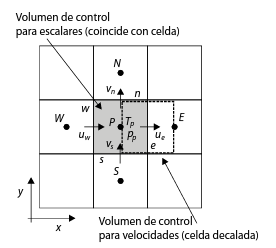
\includegraphics{33-staggeredGrid.png}
\caption{Mallado decalado (\emph{staggered grid})}
\label{fig:staggeredGrid}
\end{figure}

\subsubsection{Estabilidad numérica}\label{header-n218}

Se dice que un método numérico es \textbf{estable} cuando el proceso
iterativo converge, es decir, cuando no magnifica los errores.
Habitualmente, en las simulaciones, las iteraciones convergen de manera
lenta, pudiendo, en algunos casos, divergir. Por tanto, será útil
conocer a priori las condiciones que garanticen la convergencia de la
solución, utilizando el \textbf{análisis de estabilidad} del esquema
numérico.

A partir de las ecuaciones que rigen los flujos, no es posible llegar a
un análisis realmente exacto, sin embargo, será posible estudiarlo,
proporcionando condiciones aproximadas para la estabilidad. Una de las
más relevantes es el paso temporal máximo, \(\Delta t_{máx}\), a partir
del cual el modelo numérico se vuelve inestable (si se supera ese valor
los errores creceran exponencialmente). El paso temporal también depende
de la discretización espacial particular.

En general, se pueden establecer dos clases fundamentales de esquemas
numéricos: los \textbf{explícitos} y los \textbf{implícitos}. A partir
de la ecuación de onda se ilustra la diferenccia entre ambos:

\[\frac{\delta\phi}{\delta t}+c\frac{\delta\phi}{\delta x}=0\]

Donde \emph{c} representa la velocidad de la onda. Discretizando la
ecuación en el nodo \emph{i} y en el instante \emph{n} y planteando
diferencias finitas:

\[\frac{\phi_i^{(n)}-\phi_i^{(n-1)}}{\Delta t}+c\frac{\phi_i^{(n)}-\phi_{i-1}^{(n-1)}}{\Delta x}=0\]

Dado que la derivada espacial está evaluada en el instante anterior
\((n-1)\), por lo que se puede obtener \(\phi_i^{(n)}\) de manera
explícita en cada nodo:

\[\phi_i^{(n)}=\left[1-\left(\frac{c\Delta t}{\Delta x}\right)\right]\phi_i^{(n-1)}+\left(\frac{c \Delta t}{\Delta x}\right)\phi_{i-1}^{(n-1)}\]

Éste esquema corresponde al explícito, aunque sólo será estable si se
cumple:

\[CFL=\frac{c\Delta t}{\Delta x}\leq 1\]

donde CFL es el denominado \textbf{número de Courant}. Es común
referirse a ésta condición como la de Courant-Friedrichs-Lewy, el paso
temporal máximo se fija como aquel que permite que la velocidad de
propagación de las perturbaciones en el mallado avance como máximo el
tamaño de una celda por paso, para no perder información.

Por otro lado, en el esquema implícito, el término de la derivada
espacial se evalua en el mismo instante \emph{n} que se desea resolver:

\[\frac{\phi_i^{(n)}-\phi_i^{(n-1)}}{\Delta t}+c\frac{\phi_i^{(n)}-\phi_{i-1}^{(n)}}{\Delta x}=0\]

De este modo, se necesita resolver un sistema algebraico de ecuaciones
acoplado que calcula los valores en todos los nodos de manera
simultánea. Este esquema resulta \textbf{incondicionalmente estable}
para la ecuación de onda, independientemente del paso temporal. En este
caso el número de Courant depende del caso, siendo ventajoso elegir
números mayores que uno, siempre que la estabilidad esté garantizada.

\subsubsection{Propiedades de los métodos numéricos}\label{header-n244}

La \textbf{precisión} se relaciona de acuerdo a la solución numérica con
respecto a la solución exacta o real. No obstante, generalmente no se
conoce la solución exacta, ya que las técnicas numéricas son
aproximaciones, luego suele ser más útil referirse al error de
truncamiento de la discretización. Éste informa de cuánto se reducirá el
error si se refina la malla, si se refinase al doble se conseguiría
reducir el error de truncamiento en un factor de cuatro.

Respecto a la \textbf{consistencia}, se dice que un método numérico es
consistente si el error de truncamiento tiende a cero cuando el mallado
se va haciendo cada vez más pequeño. Garantizando la mejora de la
solución numérica obtenida.

Las dos propiedades anteriores están relacionadas con el comportamiento
del método de discretización. En cambio, la \textbf{estabilidad} es la
propiedad que controla el proceso hacia la solución. Se puede resumir
como, si el conjunto de ecuaciones resulta estable si los valores de las
variables implicadas tienden hacia una solución correcta.

El concepto de la \textbf{convergencia} determina si los valores de las
variables en los puntos del dominio tienden hacia unos valores fijados
mientras la solución progresa.

\subsection{Descripción matemática de los flujos}\label{header-n256}

Las ecuaciones de gobierno de la Mecánica de Fluidos, como las que
describen la conservación de masa, momento o energía, están expresadas
en términos de \textbf{variables específicas o intensivas}, es decir, de
cantidades expresadas por unidad de masa.

Existen dos mecanismos fundamentales responsables de la generación de un
flujo, la \textbf{difusión}, originada a nivel molecular, microescópico,
y la \textbf{convección}, asociado al movimiento del fluido a nivel
macroescópico, se puede formular los flujos en cada cara como
combinación de ambos mecanismos.

En todos los casos, el flujo debe satisfacer las tres leyes de
conservación de la mecánica más una relación de estado (termodinámica) y
las condiciones iniciales y de contorno apropiadas, es decir:

\begin{enumerate}
\def\labelenumi{\arabic{enumi}.}
\item
  Conservación de la masa (continuidad).
\item
  Conservación de la cantidad de movimiento (segunda ley de Newton).
\item
  Conservación de la energía (primer principio de la termodinámica).
\item
  Una relación de estado como \(\rho=\rho(p,T)\).
\item
  Condiciones de contorno apropiadas sobre superficies sólidas,
  entrefases, entradas y salidas.
\end{enumerate}

En el análisis integral y diferencial, estas cinco leyes están
expresadas en términos matemáticos y se resuelven mediante métodos
numéricos. En un estudio experimental, el fluido cumple de por sí estas
relaciones por tratarse de leyes fundamentales de la física.

\subsubsection{Ecuación general de
conservación}\label{header-n283}

Considérese una variable específica \(\phi\) definida sobre un volumen
de control (VC) tal y como se muentra en la figura Y. La variación
temporal de la variable en dicho volumen se puede considerar a partir
del principio de conservación como: El incremento de \(\phi\) en el VC
respecto del tiempo es igual a el flujo neto de \(\phi\) que entra en el
VC por las superficies más la generación neta de \(\phi\) en el interior
del VC respecto del tiempo.

\begin{figure}
\centering
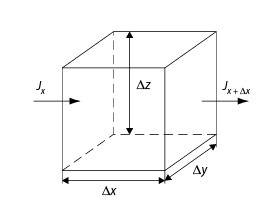
\includegraphics{34-VC.jpg}
\caption{Volumen de control}
\label{fig:VC}
\end{figure}

La expresión anterior se puede definir matemáticamente, separando los
términos difusivos de los convectivos, la forma vectorial queda:

\[\frac{\delta\left(\rho\phi\right)}{\delta t}+\triangledown\cdot\left(\rho\overrightarrow{v} \phi \right) = \triangledown \cdot \left( \Gamma \triangledown \phi \right) + S\]

Esta ecuación representa la forma conservativa (en términos de
divergencia) de la ecuación general de conservación. Cada uno de estos
términos representan (de izquierda a derecha):

\begin{itemize}
\item
  Término \textbf{temporal}, es la variación local con el tiempo en el
  interior del VC, es decir, la acumulación o disminución de \(\phi\).
\item
  Termino \textbf{convectivo}, representa el transporte de la variable
  de un punto a otro del dominio por medio de la velocidad de flujo.
\item
  Término \textbf{difusivo}, corresponde con alguno de los fenómenos de
  transporte que ocurren a nivel molecular: la ley de Fourier para la
  difusión de calor; la ley de Fick para la difusión de masa; o ley de
  Newton para la difusión de cantidad de movimiento por efectos
  viscosos.
\item
  Término \textbf{fuente}, para tener en cuenta fuentes de generación o
  destrucción de la variable transportada.
\end{itemize}

\subsubsection{Ecuaciones de gobierno para el flujo y la
transferencia de calor}\label{header-n310}

El análisis con volumenes de control es válido para cualquier flujo,
aunque a menudo se basa en propiedades "unidimensionales" o promedidas
en el contorno, siendo una herramienta muy valiosa para el análisis de
los flujos.

Todas las leyes de la mecánica están escritas para sistemas definidos
como cantidades arbitrarias de masa de identidad fija. Todo lo externo
al sistema constituye el entorno del que el sistema está separado por su
frontera o contorno. Las leyes de la mecánica establecen lo que ocurre
cuando hay una interacción entre el sistema y su entorno.

\begin{enumerate}
\def\labelenumi{\arabic{enumi}.}
\item
  El sistema se define como una cantidad fija de masa:

  \[\frac {dm}{dt}=0\]
\item
  Si el entorno ejerce una fuerza resultante \emph{F} sobre el sistema,
  la 2ª ley de Newton expresa que la masa se acelera, esto es, la
  conservación de la cantidad de movimiento:

  \[F=m \cdot a= m \frac {d\text v}{dt}= \frac {d}{dt} \left( m \text v\right)\]
\item
  Si el entorno ejerce un momento resultante \emph{M} respecto al centro
  de masas del sistema, habrá un efecto de rotación, se conoce como la
  ley de conservación del momento cinético o ecuación del momento
  cinético:

  \[M= \frac {d \text H}{dt}\]

  siendo H el momento cinético o movimiento de la cantidad de movimiento
  del sistema con respecto a su centro de masas,

  \[H= \sum \left(r\times \text v \right) \delta m\]

  nótese que se trata de una ecuación vectorial que implica tres
  ecuaciones escalares de la forma:

  \[Mx=\frac{dHx}{dt}\]
\item
  Si se comunica un calor \(\delta Q\) al sistema o éste realiza un
  trabajo \(\delta W\) sobre su entorno, la energía del sistema debe
  cambiar en una cantidad \(dE\) de acuerdo con la ecuación de
  conservación de la energía o la 1ª ley de la termodinámica:

  \[\delta Q- \delta W = d E\]

  reescribiendo la ecuación para un instante \(dt\) se tiene:

  \[\dot{Q}-\dot{W}=\frac {dE}{dt}\]
\end{enumerate}

\subsubsection{Teorema del transporte de
Reynolds}\label{header-n347}

Para convertir el análisis de un sistema en el análisis de un VC, se
deben aplicar las leyes básicas a regiones específicas en lugar de a
masas concretas. Esta conversión matemática se consigue mediante el
llamado teorema de Reynolds, aplicable a todas las leyes básicas. Las
ecuaciones definidas anteriormente (3.9), (3.10), (3.11) y (3.15) se
refieren a derivadas temporales de propiedades fluidas (m, v, H y E).
Por tanto, se necesita relacionar la derivada temporal de una propiedad
del sistema con la variación de dicha propiedad dentro de una región
concreta.

La fórmula de conversión difiere ligeramente según se trate de volúmenes
fijos, móviles o deformables:

\begin{itemize}
\item
  \textbf{El volumen de control fijo}: encierra una región estacionaria
  (la superficie de control es un concepto abstracto y no obstruye de
  ninguna forma el flujo), resaltando los esfuerzos que forman parte en
  la ecuación de cantidad de movimiento.
\item
  \textbf{El volumen de control móvil}: cuando el interés se centra en
  un objeto en movimiento, de forma que el volumen de control se mueve
  con él a la misma velocidad. El volumen de control tiene volumen fijo,
  pero se debe tener en cuenta el movimiento relativo entre el agua y el
  objeto flotante. Si el volumen es constante, este movimiento relativo
  tendrá configuración estacionaria, lo cual simplifica el análisis. Si
  el volumen es variable, el movimiento relativo será no estacionario,
  de forma que habrá dependencia temporal en los resultados, y en la
  ecuación de cantidad de movimiento aparecerán ciertos términos que
  reflejarán el carácter no inercial (acelerado) del sistema de
  referencia.
\item
  \textbf{El volumen de control deformable}: en este caso se debe tener
  en cuenta la variación del movimiento relativo en el contorno, y
  también entrará en el análisis el cambio de forma del volumen de
  control.
\end{itemize}

\subsubsection{Condiciones de contorno}\label{header-n365}

La complejidad de la mezcla de comportamientos (elípticos, parabólicos e
hiperbólicos) tiene fuerte implicaciones en la manera en que las
condiciones de controno deben introducirse en un problema
fluidodinámico, en particular en aquellas zonas en las que el flujo está
limitado por condiciones de contorno fluidas.

Al no ser posible modelar el universo por completo en CFD, es necesario
acotar el dominio, considerando tan sólo un subconjunto que incluya el
sistema que se quiere resolver numéricamente. Por lo tanto, es
imprescindible aportar la información que existe en los límites
prefijados por el dominio en referencia a las variables que se quieren
resolver. Las condiciones de contorno más comunes son:

\begin{itemize}
\item
  \textbf{Condiciones de entrada}: Estas se refieren a las condiciones
  iniciales, esto es, las distribuciones espaciales para cada variable
  (velocidad, presión y temperatura) serán conocidas en el instante
  inicial. Estas secciones a menudo están situadas en el infinito
\item
  \textbf{Condiciones enfrefase} (líquido-gas): Las condiciones más
  complejas se dan en la superficie de separación líquido-gas. Existen
  diferentes modelos para implementar la mezcla de fases, en general se
  clasifican en flujos multifásifos y los multiespecie. Los multiespecie
  presentan un campo fluidodinámico único (velocidad, temperatura, ...),
  compartido por todas las especies, mientras que los multifásicos
  pueden describirse con patrones de flujo propios para cada fase.
\item
  \textbf{Condiciones de salida}: En estos casos se supone que la
  componente difusiva del flujo normal a la frontera es cero. Por tanto,
  en las condiciones de salida no se necesita especificar el valor de
  \(\phi\), puesto que queda determinado por los procesos físicos en el
  interior del dominio y es trasnportado de forma convectiva por el
  flujo saliente. Además, se desprecia el efecto difusivo en la
  condición de salida, debido a que se supone que el flujo aguas abajo
  del dominio no tiene ninguna influencia en las características del
  flujo en el interior. Para satisfacer esta condición, las condiciones
  de contorno de salida deben cumplir que estas se sitúen en zonas tales
  que las condiciones aguas abajo no influyan en la solución.
\item
  \textbf{Condición de pared sólida impermeable}: En los contornos
  sólidos no hay deslizamiento ni salto de temperaturas, es decir, la
  componente normal a la pared de la velocidad es cero y, con lo cual,
  el flujo en la frontera se debe únicamente a mecanismos difusivos.
  Además, como la velocidad es conocida, no será necesario hacer ninguna
  corrección de presión en el algoritmo de resolución.

  Sin embargo, para la componente de velocidad paralela a la pared, la
  implementación no es tan fácil. Es necesario introducir términos
  fuente que tengan en cuenta la distancia del centroide \emph{P} a la
  pared. Así mismo, habrá que tener en cuenta si el flujo es laminar o
  turbulento en la proximidad de la pared, si la pared está fija o es
  móvil y si es isoterma o introduce una determinada transferencia de
  calor. De esta forma, en función de las características de la pared se
  deben definir distintos términos fuente específicos para la componente
  de velocidad.

  \begin{itemize}
  \item
    Estructura de la \textbf{capa límite}: En el flujo cercano a una
    pared, los efectos de la viscosidad son dominantes en una pequeña
    zona, muy próxima al contorno, denominada \emph{capa límite}. En
    condiciones de flujo turbulento, esta capa límite se divide a su vez
    en tres regiones diferenciadas: la subcapa viscosa (\emph{viscous
    sublayer}), la subcapa logarítmica (\emph{log-law region}) y la
    región esterior (\emph{outer layer}). Las dos primeras subcapas
    constituyen la región interior (\emph{inner layer}) de la capa
    límite.

    Para diferenciar cada una de las subcapas se utiliza el parámetro
    adimensionalizado \(y^+\), que se define como:

    \[y^+ = \frac{\rho u_{\tau}y}{\mu}\]

    donde \(u_{\tau}\) es la denominada \emph{velocidad de fricción}.
    Esta velocidad se determina como:

    \[u_{\tau} = \sqrt{\frac{\tau _{\text pared}}{ \rho}}\]

    siendo \(\tau _{\text pared}\) la tensión cortante en la pared. La
    velocidad de fricción se usa también para adimensionalizar la
    velocidad, fijándose así el parámetro adimensional \(u^+\) definido
    como:

    \[u^+=\frac{u}{u_{\tau}}\]
  \end{itemize}
\item
  \textbf{Condición de simetría}: Esta condición se satisface en un
  contorno cuando no se tiene flujo a través del contorno; y tampoco, se
  permite el transporte de ningún escalar a través de la superficie.
  Para implementarla en el código, se fija que las velocidades normales
  a la superficie de simetría sean cero y, respecto a los escalares, se
  igualan los valores que están contiguos fuera de la frontera, con los
  del interior del dominio.
\item
  \textbf{Condiciones periódicas y cíclicas}: Son aquellas que delimitan
  problemas que se repiten en el espacio, ya sea circunferencial o
  longitudinalmente. Si el fenómeno se repite longitudinalmente, se
  suele denominar periódicas, mientras que si se repite
  circunferencialmente, se llaman cíclicas.
\end{itemize}

\subsection{Resolución de las ecuaciones dede flujo}\label{header-n407}

Los fenómenos de convección de una variable escalar \(\phi\) dependen de
la dirección y magnitud del campo de flujo local. Para desarrollar los
métodos de discretización del término convectivo se supone la velocidad
conocida. Pero en general, el campo de velocidades se desconoce y
aparece como parte implicada en el proceso de resolución junto con el
resto de vaiables transportadas (normalmente escalares).

\subsubsection{Algoritmos de resolución}\label{header-n412}

Las estrategias más comunes para calcular el campo de flujo completo
(presiones, velocidades, temperaturas, etc.) son:

\begin{itemize}
\item
  Algoritmo \textbf{SIMPLE}: A partir de 1970 Brian Spalding inspirado
  en Patankar y Spalding, desarrolló una formulación implícita en
  términos de velocidad y presión, introduciendo por primera vez el
  método de acoplamiento SIMPLE (Semi- Implicit Method for
  Pressure-Linked Equations). Este método se utiliza, sobre todo, para
  flujos continuos y en estado estacionario.
\item
  Algoritmo \textbf{PISO}: Se trata de un método más avanzado para
  problemas transitorios. Es necesario tener un campo de presiones muy
  exacto, ya que, se requiere en el paso de la corrección de la
  velocidad para alcanzar la conservación de la masa, es decir,
  \(div(\text v)=0\). En otras palabras, si la velocidad del flujo es
  cero (por ser ortogonal a la pared) es necesario que la segunda
  derivada de la presión (ortogonal a la pared) también sea cero (en
  áreas donde la densidad es constante),
  \href{https://cfd.direct/openfoam/user-guide/fvSolution/\#x21-1170004.5}{User
  Guide: 4.5.1.1 Solution tolerances}.
\item
  Algoritmo \textbf{PIMPLE}: Una combinación de SIMPLE-PISO el cual
  emplea métodos de acoplamiento para corregir la ecuación del momento.
\end{itemize}

Con el paso del tiempo o de la solución, el algoritmo resuelve la
ecuación de la presión, para satisfacer la conservación de la masa, con
una corrección explícita para la velocidad que satisfaga la conservación
del momento. Opcionalmente se puede empezar cada paso resolviendo la
ecuación del momento, mediante el denominado \emph{momentum predictor}.

Mientras todos los algoritmos resuelven las mismas ecuaciones de
gobierno (aunque en diferentes formas), difieren principalmente en cómo
realizan el bucle sobre las ecuaciones. Detallado en la guía oficial de
OpenFOAM
\href{https://cfd.direct/openfoam/user-guide/fvSolution/\#x20-1550004.5.3}{User
Guide: 4.5.3 PISO, SIMPLE and PIMPLE algorithms}.

\subsubsection{Métodos iterativos de
resolución}\label{header-n431}

El proceso de discretización desemboca en el establecimiento de un
sistema lineal de ecuaciones algebraicas de la forma:

\[\left[A\right]\left[\phi\right]=\left[b\right]\]

donde {[}\emph{A}{]} es la matriz de coeficientes del sistema, de
dimensiones \(N\times N\) (siendo \emph{N} el número total de incógnitas
o número de celdas del mallado), \([\phi]\) es el vector con las
incógnitas y \([b]\) el vector de términos independientes (fuentes,
condiciones de contorno, etc.).

La complejidad y tamaño del sistema de ecuaciones depende de las
dimensiones del problema (1-D, 2-D o 3-D), del número de nodos de la
malla y de los esquemas de discretización empleados. Además, las
particularidades que presenta la matriz de coeficientes {[}\emph{A}{]}
obligan a que se utilice una familia de métodos muy determinada.

Una de las principales características de la matriz de coeficientes es
que es una \textbf{matriz dispersa}, esto es, está prácticamente
compuesta de ceros. Otra consideración es que en función de la
estructura de la malla y de la forma en que se defina la conectividad de
las celdas, los valores no nulos presentan distintos \textbf{patrones de
posición} en el interior de la matriz.

Los métodos de serolución de sistemas lineales de clasifican en dos
categorías:

\begin{itemize}
\item
  Los \textbf{métodos directos}, como el método de inversión de Cramer o
  la eliminación gaussiana, no aprovechan la presencia de ceros en la
  matriz de coeficientes o la estructura preferente diagonal para
  ahorrar esfuerzo de cálculo. Estos métodos, implican un número fijo de
  operaciones, que suele ser del orden de \(N^3\) (siendo N el número de
  celdas), y por tanto, requieren unas capacidades de cálculo
  inabordables. Además no hacen uso de las aproximaciones iniciales de
  la solución, luego apenas se utilizan en el contexto de las técnicas
  CFD.
\item
  Por otro lado, los \textbf{métodos iterativos} se basan en la
  aplicación repetitiva del algoritmo hasta que se asegura la
  convergencia. Normalmente, esta técnica requiere un número elevado de
  operaciones, acercandose a la solución por sucesivas aproximaciones.
  El número total de operaciones es del orden de N en cada ciclo
  iterativo, que supone unos esfuerzos computacionales asequibles a
  costa de alargar el tiempo de resolución. Estos métodos pueden ser
  reformulados para adecuarse a las características de la matriz de
  coeficientes, almacenando, tan sólo, los coeficientes no nulos de las
  ecuaciones.

  Los métodos iterativos por excelencia son los de Jacobi y
  Gauss-Seidel, fáciles de implementar, pero que convergen lentamente
  cuando el número de ecuaciones a resolver es considerable.
\end{itemize}

\subsection{Modelización de la turbulencia}\label{header-n454}

La turbulencia es un estado caótico e irregular del movimiento de un
fluido que se establece a partir de la aparición de irregularidades en
las condiciones iniciales o de contorno de la corriente fluida. Estas
inestabilidades se amplifican y se retroalimentan de forma cíclica,
creando \textbf{vórtices} (\emph{eddies}) turbulentos que se crean y se
destruyen.

La turbulencia es una característica de los flujos, su aparición exige
de la existencia de un fluido en movimiento, en el que los fenómenos de
convección (inerciales) asociados a la velocidad sean varios órdenes de
magnitud superiores a los efectos difusivos (disipativos) relacionados
con la viscosidad del fluido. Esta relación es el conocido número de
Reynolds que establece la frontera (aproximada) entre condiciones de
flujo laminar y flujo turbulento.

\subsubsection{Escalas de turbulencia: la cascada de
energía}\label{header-n461}

La turbulencia es tridimensional y contiene un amplio \textbf{espectro
de escalas} espaciales y temporales. Típicamente, los vórtices de mayor
tamaño interaccionan con el flujo principal, extrayendo energía de él.
Físicamente, esto es posible gracias a que el propio flujo convectivo
deforma esos vórtices más grandes, confiriéndoles energía en el proceso.

Richardson (1922) fue el primero en introducir el concepto de
\textbf{cascada de energía} para describir el proceso por el cual los
vórtices más grandes se dividen en estructuras más pequeñas a las cuales
pasan energía, así sucesivamente hasta llegar a las escalas puramente
disipativas. Este proceso de ruptura se produce en cascada, por lo que
en un movimiento turbulento coexisten una gran variedad de escalas,
correspondientes a los distintos tamaños de vórtices, los cuales son
arrastrados y estirados por la acción de los gradientes del flujo
promedio dominante y por si interacción con los demás vórtices. Este
proceso de división continúa hasta que la escala de los vórtices es tan
pequeña que su número de Reynolds no es lo suficiente grande como para
que la inestabilidad persista. En esos vórtices pequeños, la energía
cinética contenida en los vórtices se transforma en calor por disipación
viscosa.

\begin{figure}
\centering
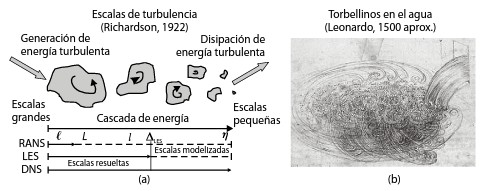
\includegraphics{35-ETurb.jpg}
\caption[Escala de la turbulencia]{Escala de la turbulencia y proceso de cascada de energía, esquema conceptual de Richardson}
\label{fig:ETurb}
\end{figure}

\subsubsection{Aproximaciones numéricas para el tratamiento de la
turbulencia}\label{header-n472}

La solución numérica para flujos turbulentos puede abordarse desde
distintos niveles de aproximación, proporcionando así descripciones del
flujo con mayor o menor detalle. Esto se consigue en función del número
de escalas de la turbulencia que se quiera resolver en la simulación, o
lo que es igual, en función de la cantidad de energía cinética
turbulenta que se vaya a transportar en las ecuaciones constitutivas.

En general, se distinguen tres aproximaciones diferentes: la simulación
numérica directa (DNS, \emph{Direct Numerical Simulation}), en la que
usa una malla extremadamente fina para poder resolver todas las escalas
de la turbulencia; la \textbf{simulación de vórtices grandes (LES,
\emph{Large Eddy Simulation})}, con mallas menos densas que permiten
resolver sólo los torbellinos grandes que transportan entre el 50 y el
80\% de toda la energía cinética turbulenta; finalmente la
\textbf{simulación de ecuaciones de NS promedidas por Reynolds (RANS,
\emph{Reynolds Average Navier-Stokes equations})} en las que todas las
escalas se modelizan mediante el uso de modelos de turbulencia.

Aunque algunos flujos sencillos se han resuelto utilizando simulación
directa (DNS) no es posible emplearla de forma sistemática para resolver
problemas industriales de interés práctico debido a su coste
computacional prohibitivo. Por esta razón se emplean habitualmente los
métodos RANS y en ciertas ocasiones las técnicas LES.

\begin{itemize}
\item
  Simulaciones directas (DNS)

  En las simulaciones directas se discretizan y resuelven las ecuaciones
  de NS en una malla suficentemente fina. La longitud característica del
  vórtice más pequeño se calcula a partir de la escala de Kolmogorov,
  \(\eta\). La relación entre \(\eta\) y la escala longitudinal \emph{L}
  del mayor vórtice es:

  \[\frac {L}{\eta} \sim (Re_L)^{\frac{3}{4}}\]

  donde \(Re_L\) es el número de Re con respecto a L. Si la dimensión
  del flujo medio es del orden \(L^3\) y el tamaño \(N_x\) de cada
  elemento de la malla es igual a \(\eta\), el número de elementos
  \(N_{elem}\) necesarios para discretizar el flujo es:

  \[N_{elem} \sim (Re_L)^{\frac{9}{4}}\]

  En aplicaciones industriales como la aerodinámica de los automóviles,
  los números de Re suelen ser sobre \(10^6\). Por tanto, la resolución
  adecuada usando DNS requeriría sobre \(10^{13}\) nodos de malla, algo
  imposible de abordar ni en paralelo por la falta de CPU
  (procesamiento).

  \begin{figure}
  \centering
  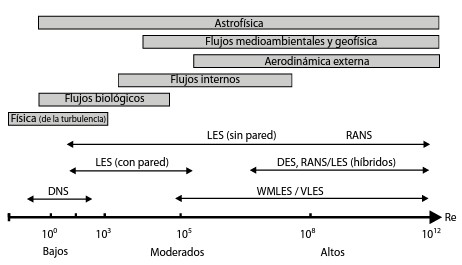
\includegraphics{36-ReTurb.jpg}
  \caption{Tipos de aproximaciones recomendadas en función del número de Re}
  \end{figure}


\item
  simulación de vórtices grandes (LES)

  Es una técnica intermedia entre DNS y RANS, en la que las
  contribuciones de las escalas grandes, portadoras de energía, y
  responsables de las estructuras de transferencia de energía y de
  momento, se resuelven en el sistema de ecuaciones, mientras que el
  efecto de las escalas más pequeñas sobre turbulencia es modelizado. Ya
  que las escalas más pequeñas tienden a ser más isotrópicas, homogéneas
  e universales, y menos afectadas por condiciones de contorno que las
  macroescalas. Su aplicación se divide en dos etapas: filtrado espacial
  de las ecuaciones (de acuerdo a un filtro típico denominado
  \(\triangle\)) y modelización de las subescalas turbulentas (SGS o
  \emph{Sub Grid Scale modelling}).

  En las simulaciones LES sólo se resuelven las escalas grandes del
  movimiento. El hecho de que las escalas intermedias transfieran su
  energía a las escalas más pequeñas (cascada de energía), así como la
  disipación viscosa venga fijada por las escalas grandes, son las
  características físicas utilizadas en esta técnica, así como en la
  definición de los modelos de submalla (\textbf{modelos SGS}).

  Desde el punto de vista matemático, estas técnicas emplean un
  \textbf{promediado espacial} de las ecuaciones de transporte mediante
  un filtro de tamaño \(\triangle\) que sirve de frontera entre las
  macroescalas a resolver y las microescalas a modelar. La gran ventaja
  de este tratamiento es que se ajusta perfectamente a las
  características fenomenológicas de ambas escalas:

  \begin{itemize}
  \item
    Los torbellinos grandes son difíciles de modelizar, puesto que
    presentan una clara anisotropía, pueden estar sujetos a efectos de
    memoria en el flujo y, sobre todo, dependen claramente de la
    geometría y del tipo de flujo principal. Luego se deberá plantear
    una técnica para cada caso que deba resolverlos y no modelarlos.
  \item
    La resolución de las pequeñas escalas exige unas discretizaciones
    extremadamente finas y costosas, inevitables para números de Re
    grandes. Sin embargo, estas escalas son típicamente isotrópicas y de
    carácter más universal, porque en el proceso de cascada los
    torbellinos han "olvidado" cuál es su procedencia. Por tanto, siendo
    sencillas de modelizar, no son necesarios grandes medios
    computacionales para su resolución.
  \end{itemize}
\item
  Simulación de ecuaciones de NS promedidas por Reynolds (RANS)

  La turbulencia se caracteriza por las fluctuaciones aleatorias que se
  superponen al valor promedio (estadístico). En la aproximación RANS se
  introduce un romediado temporal a las variables con el objeto de
  separar el valor medio del fluctuante, \(\phi =\overline{\phi}+\phi\).
  Al aplicar este promedio (flujo medio) sobre las ecuaciones de flujo,
  para el casco incompresible, se obtiene un nuevo conjunto de
  ecuaciones que pasan a describir las variables promediadas, pero que
  además contienen promedios de los productos de las componentes
  fluctuantes de la velocidad. Estos productos, las tensiones de
  Reynolds, tienen que modelarse para poder cerrar el sistema de
  ecuaciones.
\end{itemize}

\subsection{Flujos multifásicos}\label{header-n518}

El método de resolución para el transporte de flujos multiespecie
utiliza el concepto de \textbf{mezcla de fluido}. De esta forma, se
utiliza primero ese medio de mezcla como constitutivo para resolver las
ecuaciones de momento, continuidad y energía (con el valor de densidad y
viscosidad de la mezcla) y después se resuelven de manera acoplada las
ecuaciones para cada especie a partir de los campos globales obtenidos.
Así se consigue resolver un único campo fluido para toda la mezcla.

Dentro de este tipo de problemas es posible incluir muchos régimenes de
flujo diferentes, detallados en el libro de {[}Técnicas numéricas
p337{]}, entre ellos los que intervendránen el estudio son los
\textbf{flujos estratificados} o con superficie libre: es el caso de
fluidos inmiscibles, separados por una interfaz claramente definida,
como la interfaz entre el aceite y el agua o la superficie libre de
líquido en un canal hidrodinámico.

El modelo VOF permite el modelado de dos o más fluidos inmiscibles,
mediante la resolución de un único conjunto de ecuaciones para la
conservación de masa, momento y energía. La fracción de volumen de cada
una de las fases se resuelve con una ecuación de transporte, a partir de
la cual es posible definir la posición y evolución de las interfases.

Este modelo sólo es aplicable al análisis de flujos estratificados, con
superficies libres o con grandes bolsas de aire atrapadas o
transportadas en corrientes fluidas. El mayor problema es, precisamente,
el cálculo de las interfases que delimitan a cada una de las fases en el
interior del dominio.

Será necesario un algoritmo de resolución conservativo que defina las
interfases a lo largo del tiempo, procurando que la difusión numérica
esté controlada para el cálculo de los flujos de las fracciones de
volumen. Es preciso, por tanto, introducir un algoritmo que determine la
variación de \(\alpha\) (fracción de volumen de cada celda donde 0
corresponde a que el volumen de la celda es todo aire y 1 todo agua).
Existen dos métodos para reconstruir la interfase a partir de los
valores de \(\alpha\) en las celdas: cálculo de la interfaz por líneas
simples (SLIC), que aproxima la interfaz por líneas rectas paralelas a
los ejes coordenados, o el cálculo de la interfaz por aproximación de
pendientes (PLIC), que emplea líneas con pendiente para reconstruir la
interfaz.

\begin{figure}
\centering
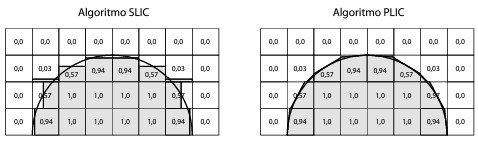
\includegraphics{37-interfase.jpg}
\caption[Algoritmos para la reconstrucción de la interfase]{Algoritmos para la reconstrucción de la interfase \cite{kothe96}}
\label{fig:interfase}
\end{figure}
